%\begin{document}

Concurrent languages can be generically classified in two major execution 
models.
%
In the \emph{asynchronous model}, the program activities (e.g. threads and 
processes) run independently of one another as result of non-deterministic 
preemptive scheduling.
In order to coordinate at specific points, these activities require explicit 
use of synchronization primitives (e.g. mutual exclusion and message passing).
%
In the \emph{synchronous model}, the program activities (e.g.  callbacks and 
coroutines) require explicit control/scheduling primitives (e.g. returning or 
yielding).
For this reason, they are inherently synchronized, as the programmer himself 
specifies how they execute and transfer control.

In this chapter we give an overview of these models, focusing on the 
synchronous model, given that \CEU and most related work targeting 
WSNs~\cite{wsn.nesc,wsn.protothreads,wsn.osm,wsn.tinythreads,wsn.sol,wsn.flowtalk,wsn.ocram} 
(detailed in Chapter~\ref{sec.related}) are synchronous.

\begin{comment}
We use this classification to give an abstract overview of related works in 
this section, although we also comment about specific languages and systems in 
our discussion.

Note that the terms synchronous and asynchronous are somewhat ambiguous, as 
they may be used in different contexts.
The reason is that \emph{synchronous languages} require \emph{asynchronous 
primitives} (i.e. non-blocking calls), while \emph{asynchronous languages} 
require \emph{synchronous primitives} (e.g. locks and semaphores).
%We use the definition of synchronous languages as found in 
%\cite{rp.twelve,rp.hypothesis}.
\end{comment}

%%%%%%%%%%%%%%%%%%%%%%%%%%%%%%%%%%%%%%%%%%%%%%%%%%%%%%%%%%%%%%%%%%%%%%%%%%%%%%%

\section{Asynchronous model}

The asynchronous model of computation can be classified according to how 
independent activities coordinate.
In \emph{shared memory} concurrency, communication is via global state, while 
synchronization is via mutual exclusion.
%Examples following this style are \emph{pthreads} and other multithreading 
%libraries.
In \emph{message passing}, both communication and synchronization happen via 
exchanging messages.

The default behavior of activities being independent hinders the development of 
highly synchronized applications.
As a practical evidence, Figure~\ref{lst.related.leds} shows a simple 
application that blinks two LEDs in parallel with different frequencies%
\footnote{The complete source code and a video demos for the application can be 
found at \url{http://www.ceu-lang.org/TR/\#blink}.}.
We implemented it in two asynchronous styles and also in \CEU.
For \emph{shared memory} concurrency, we used a multithreaded RTOS%
\footnote{\url{http://www.chibios.org/dokuwiki/doku.php?id=start}}, while for 
message passing, we used an \emph{occam} variation for 
Arduino~\cite{arduino.occam}.

\begin{figure}[t]
\begin{minipage}[t]{0.34\linewidth}
\begin{lstlisting}
// OCCAM-PI
PROC main ()
  CHAN SIGNAL s1,s2:
  PAR
    PAR
      tick(600, s1!)
      toggle(11, s1?)
    PAR
      tick(1000, s2!)
      toggle(12, s2?)
:

\end{lstlisting}
\end{minipage}
%
\begin{minipage}[t]{0.33\linewidth}
\begin{lstlisting}
// ChibiOS
void thread1 () {
  while (1) {
    sleep(600);
    toggle(11);
  }
}
void thread2 () {
  while (1) {
    sleep(1000);
    toggle(12);
  }
}

void setup () {
  create(thread1);
  create(thread2);
}

\end{lstlisting}
\end{minipage}
%
\begin{minipage}[t]{0.31\linewidth}
\begin{lstlisting}
// Ceu
par do
  loop do
    await 600ms;
    _toggle(11);
  end
with
  loop do
    await 1s;
    _toggle(12);
  end
end
\end{lstlisting}
\end{minipage}
%
\rule{14cm}{0.37pt}
\caption{ Two blinking LEDs in OCCAM-PI, ChibiOS and \CEU.\newline
{\small %\textmd{
Each line of execution in parallel blinks a LED with a fixed (but different) 
frequency.
(The LEDs are connected to I/O ports 11 and 12.)
Every 3 seconds both LEDs should light on together.
After a couple of minutes of execution, only the implementation in \CEU remains 
synchronized.
}%}
\label{lst.related.leds}
}
\end{figure}

The LEDs should blink together every 3 seconds (LCM between 600ms and 1s).
As we expected, even for such a simple application, the LEDs in the two 
asynchronous implementations lost synchronism after some time of execution.
The \CEU{} implementation remained synchronized for all tests that we have 
performed.

The implementations are intentionally naive: they just spawn the activities to 
blink the LEDs in parallel.
The behavior for the asynchronous implementations of the blinking application 
is perfectly valid, as the preemptive execution model does not ensure implicit 
synchronization among activities.
In a synchronous language, however, the behavior must be predictable, and 
loosing synchronism is impossible by design.
We used timers in this application, but any kind of high frequency input would 
also behave nondeterministically in asynchronous systems.

Note that even though the implementations are syntactically similar, with two 
endless loops in parallel, the underlying execution models between \CEU and the 
two others are antagonistic, hence, the different execution behavior.

Although this application can be implemented correctly with an asynchronous 
execution model, it circumvents the language style, as timers need to be 
synchronized in a single thread.
Furthermore, it is common to see similar naive blinking examples in reference 
examples of asynchronous systems%
\footnote{
Example 1 in the RTOS \emph{DuinOS v0.3}:
\url{http://code.google.com/p/duinos/}.\\
Example 3 in the occam-based \emph{Concurrency for Arduino v20110201.1855}:
\url{http://concurrency.cc/}.
}, suggesting that LEDs are really supposed to blink synchronized, a guarantee 
that the language cannot provide.

%%%%%%%%%%%%%%%%%%%%%%%%%%%%%%%%%%%%%%%%%%%%%%%%%%%%%%%%%%%%%%%%%%%%%%%%%%%%%%%

\section{Synchronous model}

In this section, we present a review of some synchronous languages and 
programming techniques that more closely relate to \CEU.
%
We refer back to them in detail in Chapter~\ref{sec.related} to discuss 
specific features and differences that require a deeper knowledge about \CEU.

\textbf{Event-driven programming}

At the lowest abstract level of the synchronous model, event-driven programming 
is usually employed as a technique in general-purpose languages with no 
specific support for reactivity.
Because a single line of execution and stack are available, programmers need to 
deal with the burden of manual stack management and inversion of 
control.~\cite{sync_async.cooperative}

In the context of WSNs, the programming language \nesc~\cite{wsn.nesc} offers 
event-driven programming for the TinyOS operating system.
The concurrency model of \nesc is very flexible, supporting the traditional 
serialization among callbacks (the default and recommended behavior), and also 
asynchronous callbacks that interrupt others.
To deal with race conditions, \nesc supports atomic sections with a similar 
semantics to mutual exclusion in asynchronous languages.
We use \nesc as the back end of \CEU for TinyOS~\cite{wsn.tos}.

\textbf{Cooperative multithreading}

Cooperative multithreading is an alternative approach to preemptive 
multithreading where the programmer is responsible for scheduling activities in 
the program (known as \emph{coroutines}~\cite{lua.coroutines}).
With this approach, there are no possible race conditions on global variables, 
as the points that transfer control in coroutines are explicit (and, 
supposedly, are never inside critical sections).

In the context of WSNs, Protothreads \cite{wsn.protothreads} offer very 
lightweight cooperative multithreading for embedded systems.
Its stackless implementation reduces memory consumption but precludes support 
for local variables.
Furthermore, Protothreads provide no static safety warranties: programs can 
loop indefinitely, and accesses to globals are unrestricted.

\begin{comment}
Coroutines are similar to \CEU trails, as they both offer multiple sequential 
lines of execution to handle concurrent activities.
However, \CEU's \code{par/and} and \code{par/or} composition statements offer a 
powerful abstraction to avoid manual bookkeeping of activities, such as 
creating, starting, rejoining, and destroying them.
Also, the semantics for rejoins in parallel compositions is fundamental for the 
temporal analysis of \CEU, which cannot be done effectively with coroutines.
\end{comment}

\textbf{Finite state machines}

The use of finite state machines (FSMs) is a classic technique to implement
reactive applications, such as network protocols and graphical user interfaces.
A contemporary work~\cite{wsn.osm} targets WSNs and is based on the Statecharts 
formalism \cite{statecharts.visual}.

FSMs have some known limitations.
For instance, writing purely sequential flow is tedious, requiring to break 
programs in multiple states with a single transition connecting each of them.  
Another inherent problem of FSMs is the state explosion phenomenon, which can 
be alleviated in some designs that support hierarchical FSMs running in 
parallel \cite{wsn.osm}.
%However, adopting parallelism precludes the use of shared state, or at least 
%requires a static analysis such as that of \CEU.

%- mostrar a saida de quantos dfa tem cada um dos exemplos
%- ship tem que tirar o async
%- dizer que um programa equivalente teria esse mesmo numero de estados
%e seria impossivel de programar

%- possibly graphical languages (fosters visual) (inherent)

\textbf{Synchronous languages}

The family of reactive synchronous languages%
\footnote{
The term \emph{synchronous} is convoluted here:
\emph{Synchronous languages} evidently follow the \emph{synchronous programming 
model}, but multi-purpose languages (e.g., $Java$ and $C$) can also behave 
synchronously by applying techniques such as event-driven programming and state 
machines.
}
is an established alternative to $C$ in the field of safety-critical embedded 
systems \cite{rp.twelve}.
%
Two major styles of synchronous languages have evolved:
in the \emph{control}--\emph{imperative} style (e.g. Esterel 
\cite{esterel.design}), programs are structured with control flow primitives, 
such as parallelism, repetition, and preemption;
in the \emph{dataflow}--\emph{declarative} style (e.g. Lustre 
\cite{lustre.ieee91}), programs can be seen as graphs of values, in which a 
change to a value is propagated through its dependencies without explicit 
programming.

\CEU is strongly influenced by Esterel~\cite{esterel.ieee91} in its support for 
hierarchical compositions of activities and reactivity to events.
%
However, some fundamental differences exist, and we discuss them in detail in
Section~\ref{sec.ceu.esterel}.

\section{Programming models in WSNs}
\label{sec.ceu.overview}

A WSN application has to handle a multitude of concurrent events, such as 
timers and packet transmissions, keeping track of them according to its 
specification.
%
From a control perspective, programs are composed of two main patterns: 
\emph{sequential}, i.e., an activity with two or more sub-activities in 
sequence;
and \emph{parallel}, i.e., unrelated activities that eventually need to 
synchronize.
%
As an example, an application that alternates between sampling a sensor and 
broadcasting its readings has a sequential pattern (with an enclosing loop); 
while using a 1-minute timeout to interrupt an activity denotes a parallel 
pattern.

\begin{figure*}[!t]
%\rule{14cm}{0.37pt}
\begin{minipage}[t]{0.50\linewidth}
\begin{lstlisting}[title=\emph{/* nesC */}]
|{\color{darkgreen}\textbf{event void} Boot.booted() \{}|
  |{\color{darkblue}\textbf{call} T1.start(0)}|
  |{\color{darkpur}\textbf{call} T2.start(60000)}|
|{\color{darkgreen}\}}|
|{\color{darkblue}\textbf{event void} T1.fired() \{}|
  |{\color{darkblue}\textbf{static int} on = 0;}|
  |{\color{darkblue}\textbf{if} (on) \{}|
    |{\color{darkblue}\textbf{call} Leds.led0Off();}|
    |{\color{darkblue}\textbf{call} T1.start(1000);}|
  |{\color{darkblue}\} \textbf{else} \{}|
    |{\color{darkblue}\textbf{call} Leds.led0On();}|
    |{\color{darkblue}\textbf{call} T1.start(2000);}|
  |{\color{darkblue}\}}|
  |{\color{darkblue}on = !on}|
|{\color{darkblue}\}}|
|{\color{darkpur}\textbf{event void} T2.fired() \{}|
  |{\color{darkred}\textbf{call} T1.cancel();}|
  |{\color{darkred}\textbf{call} Leds.led0Off();}|
  |{\color{darkred}<...> // CONTINUE}|
}

\end{lstlisting}
\end{minipage}
%
%\hfill \vrule \hfill
%\hspace{0.0cm}
%
\begin{minipage}[t]{0.50\linewidth}
%\fbox{
\begin{lstlisting}[title=\emph{/* Protothreads */}]
|{\color{darkgreen}\textbf{int} main() \{}|
  |{\color{darkblue}\textbf{PT\_INIT(\&blink);}}|
  |{\color{darkpur}timer\_set(\&timeout,60000);}|
  |{\color{darkred}\textbf{while} (}|
    |{\color{darkred}\textbf{PT\_SCHEDULE}(blink()) \&\&}|
    |{\color{darkred}!timer\_expired(timeout)}|
  |{\color{darkred});}|
  |{\color{darkred}leds\_off(LEDS\_RED);}|
  |{\color{darkred}<...> // CONTINUE}|
|{\color{darkred}\}}|
|{\color{darkblue}\textbf{PT\_THREAD} blink() \{}|
  |{\color{darkblue}\textbf{while} (1) \{}|
    |{\color{darkblue}leds\_on(LEDS\_RED);}|
    |{\color{darkblue}timer\_set(\&timer,2000);}|
    |{\color{darkblue}\textbf{PT\_WAIT}(expired(\&timer));}|
    |{\color{darkblue}leds\_off(LEDS\_RED);}|
    |{\color{darkblue}timer\_set(\&timer,1000);}|
    |{\color{darkblue}\textbf{PT\_WAIT}(expired(\&timer));}|
  |{\color{darkblue}\}}|
|{\color{darkblue}\}}|
\end{lstlisting}
%}
\end{minipage}
%
%\hfill \vrule \hfill
%\hspace{0.0cm}
%
\begin{minipage}[t]{0.50\linewidth}
%\fbox{
\begin{lstlisting}[title=/* \CEU */]
|\textbf{\color{darkgreen}par/or do}|
   |\textbf{\color{darkblue}loop do}|
      |{\color{darkblue}\_Leds\_led0On();}|
      |{\color{darkblue}await 2s;}|
      |{\color{darkblue}\_Leds\_led0Off();}|
      |{\color{darkblue}await 1s;}|
   |\textbf{\color{darkblue}end}|
|\textbf{\color{darkgreen}with}|
   |{\color{darkpur}\textbf{await} 1min;}|
|\textbf{\color{darkgreen}end}|
|{\color{darkred}\_Leds\_led0Off();}|
|{\color{darkred}<...> // CONTINUE}|
\end{lstlisting}
%}
\end{minipage}
%
%\hfill \vrule \hfill
%\hspace{0.0cm}
%
\begin{minipage}[t]{0.50\linewidth}
\vspace{30pt}
\centering
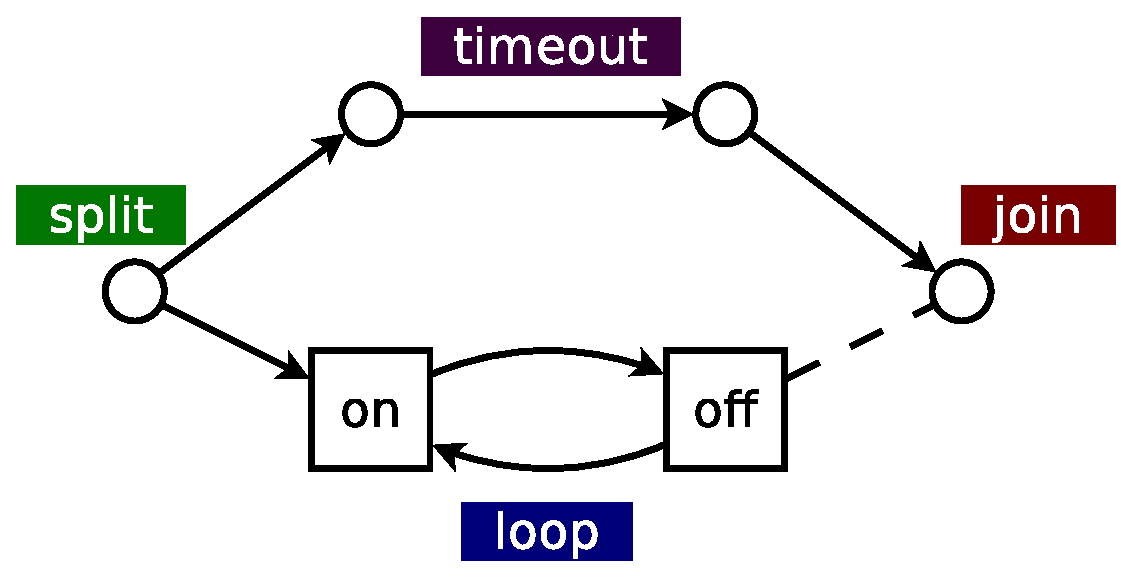
\includegraphics[width=\textwidth]{dia}
\end{minipage}
%%
%\hspace{0.0cm}
%%
\rule{14cm}{0.37pt}
\caption{ ``Blinking LED'' in
    nesC,
    Protothreads,
    and \CEU. %\newline
%{\small
%The colors associate chunks of code with respective actions in the diagram.
%}
\label{lst.all}
}
\end{figure*}

Figure~\ref{lst.all} presents the three synchronous programming (sub-)models 
commonly used in WSNs through a simple concurrent application.
It shows the implementations in \emph{nesC}~\cite{wsn.nesc}, 
\emph{Protothreads}~\cite{wsn.protothreads}, and \CEU for an application that 
continuously turns on a LED for 2 seconds and off for 1 second.
After 1 minute of activity, the application turns off the LED and proceeds to 
another activity (marked in the code as \code{<...>}).
The diagram on the bottom-right of Figure~\ref{lst.all} describes the overall 
control behavior for the application.
The sequential programming pattern is represented by the LED alternating between 
the two states, while the parallel pattern is represented by the 1-minute 
timeout.
% that interrupts the blinking LED.

The first implementation, in \emph{nesC}, which represents the 
\emph{event-driven} model, spawns two timers ``in parallel'' at boot time 
(\code{Boot.booted}): one to make the LED blink and another to wait for 1 
minute.
The callback \code{T1.fired} continuously toggles the LED and resets the timer 
according to the state variable \code{on}.
The callback \code{T2.fired} executes only once, canceling the blinking timer, 
and proceeds to \code{<...>}.
Overall, we argue that this implementation has little structure: the blinking 
loop is not explicit, but instead relies on a static state variable and 
multiple invocations of the same callback.
Furthermore, the timeout handler (\code{T2.fired}) requires specific knowledge 
about how to stop the blinking activity, and the programmer must manually 
terminate it (\code{T1.cancel()}).

The second implementation, in \emph{Protothreads}, which represents the 
\emph{multi-threaded} model~\cite{wsn.protothreads,wsn.mantisos}, uses a 
dedicated thread to make the LED blink in a loop.
This brings more structure to the solution.
The main thread also helps a reader to identify the overall sequence of the 
program, which is not easily identifiable in the event-driven implementation 
without tracking the dependencies among callbacks.
However, it still requires much bookkeeping for initializing, scheduling and 
rejoining the blinking thread after the timeout (inside the \code{while} 
condition).

% ASYNC MT?

The third implementation, in \CEU, which represents the 
\emph{synchronous-language model}, uses a \code{par/or} construct to run the 
two activities in parallel:
an endless loop to blink the LED, and a single statement that waits for 1 
minute before terminating.
The \code{par/or} stands for \emph{parallel-or} and rejoins automatically when 
any of its trails terminates.
%
We argue that the hierarchical structure of \CEU more closely reflects the 
control diagram and ties the two activities together, implying that
(a) they can only exist together;
(b) they always start together
(c) they always terminate together.
%
Besides the arguably cleaner syntax, the additional control-flow information 
that can be inferred from the program is the base for all features and safety 
guarantees introduced by \CEU.

% TODO
%The challenge is how to provide a design that embraces/xxx safety/determinism, 
%specially considering pointers
